\UNsection{1.1 - Borel's Normal Number Theorem}
\seteqgroup{1}

Consider trying to analyze the frequency of heads and tails for an infinite number of coin tosses. Because academia must remain inaccessible to those without a lexile score in the 80th percentile, and arguably less for the sake of $\boldsymbol{``}$\textit{Mathematical Rigor}$\boldsymbol{"}$  Billingsley chooses to model this infinite sequence of coinflips as a so-called \textbf{ nonterminating dyadic expansion} of the form:
\begin{UNequation}
	\omega=\sum^{\infty}_{n=1}\frac{d_n(\omega)}{2^n}=.d_1(\omega)d_2(\omega)\cdots 
\end{UNequation}
That is basically just a really fancy way of saying it is an infinite sequence of ones and zeros \textemdash the finite case of this problem conforms with the familiar binomial distribution. However, this dyadic representation is cumbersome, it is often useful to use the \textbf{Rademacher Function} which is defined as:
\begin{UNequation}
	r_n(\omega) = 2d_n(\omega) - 1 = 
	\begin{cases}
		+1 & \text{if } d_n(\omega) = 1, \\
		-1 & \text{if } d_n(\omega) = 0. 
	\end{cases}
\end{UNequation}

\vspace{-4ex}
\begin{figure}[H]
    \centering
    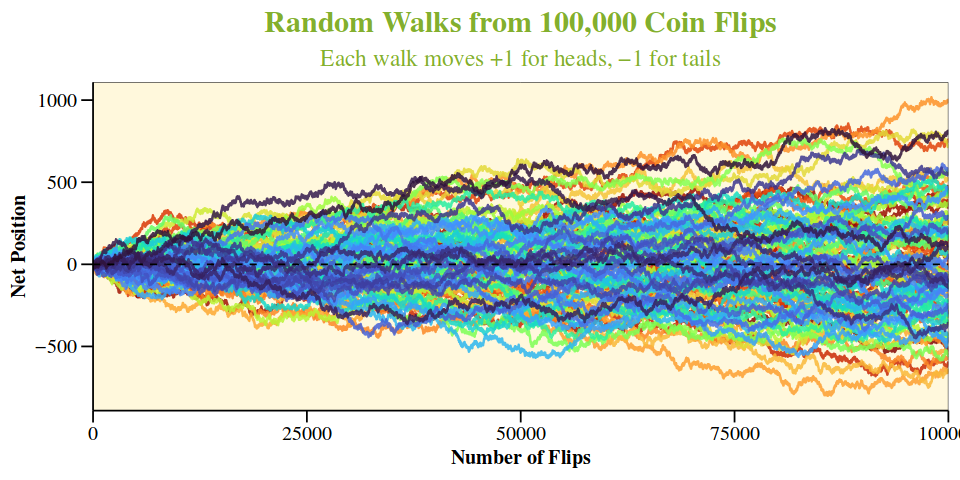
\includegraphics[width=\linewidth]{coinflip.png}
\end{figure}

Which yields the following partial sum:


\vspace{-7ex} \begin{UNequation}
	\hspace{5cm}
	s_n(\omega) = \sum_{i=1}^{n} r_i(\omega).
\end{UNequation}
\vspace{-2ex}
If \( f(\omega) \) is a step function taking value \( c_j \) in the interval \( (x_{j-1}, x_j] \), where \( 0 = x_0 < x_1 < \cdots < x_k = 1 \), then its integral in the sense of Riemann has the value
\vspace{-2ex}
\begin{UNequation}
\int_0^1 f(\omega) \, d\omega = \sum_{j=1}^k c_j (x_j - x_{j-1}).
\end{UNequation}

\UNsubsection{The Weak Law of Large Numbers} \quad
\needspace{6\baselineskip}
\textbf{Theorem 1.1:} For each $\varepsilon>0$,
\begin{UNequation}
	\lim_{n\to\infty}P\left[\omega : \left| \frac{1}{n}\sum^n_{i=1}d_i(\omega)-\frac{1}{2} \right| \geq \varepsilon \right] = 0  
\end{UNequation}
\vspace{-3ex}

\textbf{Proof:}
\begin{proofline}
	First things first, let us put this equation in a form that is easier to prove. Since \(\sum_{i=1}^n d_i(\omega) = \frac{s_n(\omega) + n}{2}\), (1.4) with \(\varepsilon/2\) in place of \(\varepsilon\) is the same thing as
	\begin{UNequation}
		\lim_{n \to \infty} P\left[ \omega : \left| \frac{1}{n}s_n(\omega) \right| \geq \varepsilon \right] = 0.
	\end{UNequation}
	Then, since this is a step function we know it must be of the following form:
	\begin{UNequation}
		\int_0^1 f(\omega)\, d\omega = \sum_{j=1}^k c_j (x_j - x_{j-1}).
	\end{UNequation}
	Thus, the total length of the interval is $\frac{1}{2}$ meaning that:
	\begin{UNequation}
		\int_0^1s_n(\omega)d\omega=0
	\end{UNequation}
	Applying \textit{Chebyshev's Inequality} to (1.5) yields:
	\begin{UNequation}
		P[\omega: \left| s_n(\omega)\right|\geq n\varepsilon  ] \leq \frac{1}{n^2\varepsilon^2}\int_0^1 s_n^2(\omega)d\omega=\frac{1}{n\varepsilon^2}
	\end{UNequation}
	This inequality results from the finite union of intervals of a step function and an application of \textit{Markov's Inequality}; this application is formally defined in the following lemma. \hfill \qed
\end{proofline}

\needspace{6\baselineskip}
Let $\Omega$ denote the unit interval $(0,1]$ if the intervals \( I_i = (a_i, b_i] \) are disjoint and are contained in \( \Omega \), assign to \( A \) the probability
\begin{UNequation}
    P(A) = \sum_{i=1}^n |I_i| = \sum_{i=1}^n (b_i - a_i).
\end{UNequation}


\textbf{Lemma:} If f is a nonnegative step function, then $[\omega: f(\omega) \geq \alpha]$  is for $\alpha > 0$
a finite union of intervals, and
\begin{UNequation}
	P[\omega:f(\omega)\geq \alpha] \leq \frac{1}{\alpha}\int_0^1f(\omega)d\omega
\end{UNequation}

That is, the probability that the number of 1s in the sequence is greater than a number $\alpha$ is less than or equal to 1 over $\alpha$ times the expected number of 1s in the sequence.\\
\textbf{Proof: }
\begin{proofline}
    The set in question is the union of the intervals \( (x_{i-1}, x_i] \) for which \( c_i \geq a \). If \( \sum' \) denotes summation over those \( i \) satisfying \( c_i \geq a \), then
    \begin{UNequation}
    P[\omega : f(\omega) \geq a] = \sum\nolimits' (x_i - x_{i-1})    
    \end{UNequation}
    by the definition (1.9). On the other hand, since the \( c_i \) are all nonnegative by hypothesis, (1.10) gives
    \begin{UNequation}
    \begin{aligned}
    \int_0^1 f(\omega)\, d\omega &= \sum_{i=1}^k c_i(x_i - x_{i-1}) \geq \mathop{\sum\nolimits'}_{j=1} c_i(x_i - x_{i-1})\\
    &\geq \sum\nolimits' a(x_i - x_{i-1}).    
    \end{aligned}
    \end{UNequation}
    \hfill \qed
\end{proofline}


\UNsubsection{The Strong Law of Large Numbers} \quad

is a special case of whats called \textbf{Borel's Normal Number Theorem}. Furthermore, the actual meat of this theorem cannot be adequately expressed in the familiar discrete probability theory. Consider the set:
\begin{UNequation}
	N=\left[\omega:\lim_{n\to\infty}\frac{1}{n}\sum_{i=1}^nd_i(\omega)=\frac{1}{2} \right]
\end{UNequation}
The points within (1.14) are called \textbf{Normal Numbers}. We want to show that a real number $\omega$ drawn from the unit interval at random is practically certain to be a normal number, which means that there is practical certainty that the asymptotic relative frequency of 1s in the sequence is equal to $\frac{1}{2}$\\[-10pt]


Before we can proceed, we need to formalize practical certainty through the idea of a negligible subset. A subset \( A \subset \Omega \) is called \textbf{negligible} if for every \( \varepsilon > 0 \), there exists a finite or countable collection of intervals \( I_1, I_2, \ldots \) such that:
\begin{UNequation}
	A \subset \bigcup_k I_k, \quad \text{and}  \quad  \sum_k |I_k| < \varepsilon.    
\end{UNequation}
A negligible set is one that can be covered by intervals the total sum of which lengths can be made arbitrarily small. From this we can then say that it is practically impossible that the random $\omega$ will lie in $A$ if $A$ is negligible, and regard it as practically certain that $\omega$ will lie in $A$ if its complement $A^c$ is negligible.\\[-10pt]

An important consequence of this is that a set consisting of a single point is clearly negligible, and so every countable set is also negligible; this is why the cumulative density function of a single point of a continuous probability distribution is zero. In the case of our infinite sequence of coin tosses this can be interpreted as saying that it is practically impossible to toss a coin infinitely many times and correctly predict the \textit{exact} sequence that the tosses will follow. \\[-10pt]

With these preliminaries in place, we can now move on to defining and proving our next theorem.


\UNsubsection{Borel's Normal Number Theorem} \quad

\textbf{Theorem 1.2:} The set of normal numbers has negligible complement.\\[-10pt]

\textbf{Proof:} 
\begin{proofline}
	\begin{UNequation}
		N=\left[\omega:\lim_{n\to\infty}\frac{1}{n}\sum_{i=1}^nd_i(\omega)=\frac{1}{2} \right]=\left[\omega:\lim_{n\to\infty}\frac{1}{n}s_n(\omega)=0 \right]
	\end{UNequation}
	To prove that $N^c$ is negligible we need to show that $A=N^c$ satisfies the two conditions defined by (1.15). We begin by applying (1.9) where $f(\omega)=s_n^4(\omega)$ and $\alpha =  n^4\varepsilon^4$
	\begin{UNequation}
		P\left[\omega: |s_n(\omega)|\geq n\varepsilon \right] \leq \frac{1}{n^4\varepsilon^4}\int_0^1s_n^4(\omega)d\omega
	\end{UNequation}
	Since $s_n^4(\omega)$ is simply our partial sum raised to the fourth power we can equivalently express it as the sum of four Rademacher functions multiplied together where each of the respective indices ($\alpha$, $\beta$, $\gamma$, $\delta$) range from 1 to n.
	\begin{UNequation}
		s_n^4(\omega)=\sum r_\alpha(\omega)r_\beta(\omega)r_\gamma(\omega)r_\delta(\omega)
	\end{UNequation}
	This sum can be simplified by combining like terms to produce a new equation in which the indices are distinct. This yields an equation of one of the following forms depending on how the indices cancel with one another.
	\begin{UNequation}
		s_n^4(\omega)\left\{
		\begin{aligned}
			  & r_i^4(\omega) = 1,                                                     \\
			  & r_i^2(\omega)\, r_j^2(\omega) = 1,                                     \\
			  & r_i^2(\omega)\, r_j(\omega)\, r_k(\omega) = r_j(\omega)\, r_k(\omega), \\
			  & r_i^3(\omega)\, r_j(\omega) = r_i(\omega)\, r_j(\omega),               \\
			  & r_i(\omega)\, r_j(\omega)\, r_k(\omega)\, r_l(\omega).                 
		\end{aligned}
		\right.
	\end{UNequation}
	This is a linear system of equations, evidently the first two forms integrate to one. Each of the subsequent forms, however, becomes an odd function over sub-intervals due to alternation of the highest index function. These last three forms integrate to zero since integrating an odd function over symmetric intervals results in cancellation.\\[-10pt]
	
	The first form corresponds to the case where all 4 indices are equal, meaning there is effectively a single index that runs from 1 to $n$ giving us $n$ possible terms. The second form corresponds to the case where there is effectively 2 distinct indices. However, since there are three different ways to produce each pair of distinct indices the number of possible terms contributed by the second form is equal to: 
	\begin{UNequation}
		3\cdot \binom{n}{2} = 3 \cdot \frac{\xcancel{2}n(n-1)}{\xcancel{2}} = 3n(n-1)
	\end{UNequation}
	
	
	We can then integrate $s_n^4(\omega)$ term by term, which yields:
	\begin{UNequation}
		\int_0^1s_n^4(\omega)d\omega=n+3n(n-1)\leq 3n^2
	\end{UNequation}
	Substituting this simplified expression into (1.17) gives the following:
	\begin{UNequation}
		P\left[\omega: \left| \frac{1}{n}s_n(\omega) \right| \geq \varepsilon \right] \leq \frac{3}{n^2\varepsilon^4}
	\end{UNequation}
	Fix a positive sequence $\{\varepsilon_n\}$ tending to $0$ slowly enough so that the following series converges.
	\begin{UNequation}
		\sum_n \varepsilon_n^{-4} n^{-2}
	\end{UNequation}
	
	\vspace{-5ex}
	
	Now define the sets:
	\begin{UNequation}
		\begin{aligned}
			  & \begin{array}{l} 
			A_n = \left\{ \omega : \left| \frac{1}{n} s_n(\omega) \right| \geq \varepsilon_n \right\}
			\end{array}
			\quad \& \quad
			\begin{array}{l}
			P(A_n) \leq 3 \varepsilon_n^{-4} n^{-2},\\
			\sum_n P(A_n) < \infty
			\end{array}
		\end{aligned}
	\end{UNequation}
	
	
	If for some $m$,\\
	$\omega \in A_n^c$ for all $n \geq m$, then
	\vspace{-7ex}
	\begin{UNequation}
		\hspace{4cm}
		\begin{aligned}
			  & \begin{array}{l} 
			\hspace{4cm}
			\end{array}
			\quad
			\begin{array}{l}
			\scalebox{1.25}[1.25]{$\left| \frac{1}{n} s_n(\omega) \right| < \varepsilon_n$} \quad \text{{\footnotesize for all $n \geq m$}}
			\end{array}
		\end{aligned}
	\end{UNequation}
	
	and since $\varepsilon_n \to 0$, it follows that $\omega$ is a normal number.
	
	Thus, for each $m$,
	\begin{UNequation}
		\bigcap_{n=m}^\infty A_n^c \subseteq N \quad { \text{\footnotesize or equivalently}} \quad
		N^c \subseteq \bigcup_{n=m}^\infty A_n.
	\end{UNequation}
	
	This last inclusion leads directly to the required covering.
	
	Given any $\varepsilon > 0$, choose $m$ so that
	\begin{UNequation}
		\sum_{n=m}^\infty P(A_n) < \varepsilon.
	\end{UNequation}
	
	Each set $A_n$ is a finite disjoint union of dyadic intervals:
	\begin{UNequation}
		A_n = \bigcup_k I_{nk}, \quad \sum_k |I_{nk}| = P(A_n).
	\end{UNequation}
	
	
	Therefore, the union
	\begin{UNequation}
		\bigcup_{n=m}^\infty A_n = \bigcup_{n=m}^\infty \bigcup_k I_{nk}
	\end{UNequation}
	is a countable union of intervals (not necessarily disjoint), with
	\begin{UNequation}
		\sum_{n=m}^\infty \sum_k |I_{nk}| = \sum_{n=m}^\infty P(A_n) < \varepsilon.
	\end{UNequation}
	
	Hence, the collection of intervals $\{ I_{nk} : n \geq m, k \geq 1 \}$ provides a covering of $N^c$ satisfying
	\begin{UNequation}
		N^c \subseteq \bigcup I_{nk}, \quad \sum |I_{nk}| < \varepsilon,
	\end{UNequation}
	which is exactly the form required by the definition of negligibility (as given in equation (1.11)). \hfill \qed 
\end{proofline}

\UNsubsection{Length and Negligibility} \quad

The next theorem will act as our entry point for defining measure. These three statements taken together ensure the additivity of disjoint events that we expect within a sample space. In discrete probability this is a result of the properties of the Riemann integral. However, theorem 1.3 provides us with a way to guarantee the additivity of disjoint events independent of the Riemann integral, allowing us to generalize beyond the restrictive assumptions of Riemann integration.\\[10pt]

\needspace{14\baselineskip}
\textbf{Theorem 1.3: } Let $I = (a, b]$ be an interval of length $|I| = b - a$ and,\\
let $I_k = (a_k, b_k]$ be a finite or infinite sequence of bounded intervals (they need not be subintervals of $(0,1]$). Then:

\begin{enumerate}[label=\textbf{\roman*.}, topsep=0pt, itemsep=-3pt]
	\item If $\bigcup_k I_k \subset I$, and the $I_k$ are disjoint, then $\sum_k |I_k| \leq |I|$.
	\item If $I \subset \bigcup_k I_k$ (the $I_k$ need not be disjoint), then $|I| \leq \sum_k |I_k|$.
	\item If $I = \bigcup_k I_k$, and the $I_k$ are disjoint, then $|I| = \sum_k |I_k|$.
\end{enumerate}

\textbf{Proof:}
\begin{proofline}
	To begin, we can observe that \textbf{iii.} follows from \textbf{i.} \& \textbf{ii.} so we just need to prove the first two claims:\\
	{\footnotesize \textbf{Proof of i:}}
	\vspace{-1.5ex}
	\begin{proofline}[1em]
		{\footnotesize \textbf{Finite Case:}} Assume that there are $n$ intervals. The result clearly holds if $n=1$, we assume that it holds for $n-1$. If $a_n$ is the largest among $a_1,...,a_n$, then $\bigcup_{k=1} I_{n-1}(a_k, b_k] \subset (a, a_n)$, so that $\sum_{k=1}^{n-1}(b_k-a_k) \leq a_n -a $ by induction, and thus $\sum_{k=1}^{n}(b_k-a_k) \leq a_n -a + (b_n-a_n) \leq b-a$.\\[5pt]
		{\footnotesize \textbf{Infinite Case:}} If there are an infinite amount of intervals, we just showed that any finite subcollection must satisfy \textbf{i.}, as a result $\sum_{k=1}^{n}(b_k-a_k) \leq b-a$, and since $n$ is arbitrary this holds in the infinite case.
	\end{proofline}
	    
	{\footnotesize \textbf{Proof of ii:}}
	\vspace{-1.5ex}
	\begin{proofline}[1em]
		{\footnotesize \textbf{Finite Case:}} Assume that \textbf{ii.} holds for the case of $n-1$ intervals and that $(a,b] \subset \bigcup_{k=1}^n(a_k,b_k]$ where $a_n < b \leq b_n$. If $a_n \leq a$, then the result clearly holds. Otherwise, $(a,a_n] \subset \bigcup_{k=1}^{n-1}(a_k, b_k]$, so that $\sum_{k=1}^{n-1}(b_k-a_k) \geq a_n - a$ by induction. Thus, $\sum_{k=1}^n(b_k-a_k) \geq (a_k-a)+(b_n-a_n) \geq b-a$. The finite case follows from this by induction.\\[5pt]
		{\footnotesize \textbf{Infinite Case:}} Assume that  $(a,b] \subset \bigcup_{k=1}^{\infty}(a_k, b_k]$. If $0 < \varepsilon < b - a$, the open intervals $(a_k, b_k + \varepsilon2^{-k})$ cover the closed interval $[a + \varepsilon, b]$, and it follows by the \textit{Heine-Borel theorem} that $(a + \varepsilon, b] \subset \bigcup_{k=1}^n(a_k, b_k + \varepsilon2^{-k}]$, meaning that by the finite case we have $b - (a + \varepsilon) \leq \sum_{k=1}^n(b_k + \varepsilon 2^{-k}-a_k) \leq \sum_{k=1}^{\infty}(b_k-a_k) + \varepsilon$. Thus, since $\varepsilon$ is arbitrarily small the infinite case follows.
			\end{proofline}
			\vspace{-4ex}
			\hfill \qed
			\end{proofline}
			Part \textbf{ii.} of theorem 1.3 proves the fact that an interval which has  positive length cannot be negligible. The intuition behind this fact follows directly from our definition of a negligible interval being one that can be made arbitrarily small. Any interval of positive length cannot be made smaller than its length, and therefore cannot be negligible. However, in order to rigorously prove this fact we can defer to the intrinsic properties of the real numbers.
			
			
			
